%!TEX TS-program = pdflatex
%!TEX encoding = UTF-8 Unicode



    %                     %            %
    %                                  %
    %                                  %
   %%%    %%%%   %%%%%   %%           %%%    %%%%  %    %
    %    %    % %         %            %    %    %  %  %
    %    %%%%%%  %%%%     %            %    %%%%%%   %%
    %    %           %    %            %    %        %%
    %    %           %    %     %%     %    %       %  %
     %%   %%%%% %%%%%    %%%    %%      %%   %%%%% %    %



         %%%%%%%%%%%%%%%%%%%%%%%%%%%%%%%%%%%%%%%%
         %                                      %
         %  "Scheletro" di una tesi di laurea   %
         %           (in Matematica)            %
         %      dell'Universita` di Udine       %
         %                                      %
         %%%%%%%%%%%%%%%%%%%%%%%%%%%%%%%%%%%%%%%%

              %%%%%%%%%%%%%%%%%%%%%%%%%%%%
              %  Autore: Gianluca Gorni  %
              %%%%%%%%%%%%%%%%%%%%%%%%%%%%

   %%%%%%%%%%%%%%%%%%%%%%%%%%%%%%%%%%%%%%%%%%%%%%%%%%%%%
   %%%%%   Ultima modifica:  10 luglio 2016        %%%%%
   %%%%%%%%%%%%%%%%%%%%%%%%%%%%%%%%%%%%%%%%%%%%%%%%%%%%%



                                 %            %%
                                 %             %
   %%%%  % %%   %%%   %%%% %%%%  %%%%   %%%    %    %%%
   %   % %%  % %   % %   % % % % %   % %   %   %   %   %
   %   % %     %%%%% %   % % % % %   % %   %   %   %   %
   %   % %     %     %  %% % % % %   % %   %   %   %   %
   %%%%  %      %%%%  %% % % % % %%%%   %%%   %%%   %%%
   %
   %




  %%%%%%%%%%%%%%%%%%%%%%%%%%%%%%%%%%%%%%%%%%%%%%%%%%%%%%%%%
  % Usare una versione di LaTeX con sillabazione italiana %
  %%%%%%%%%%%%%%%%%%%%%%%%%%%%%%%%%%%%%%%%%%%%%%%%%%%%%%%%%

\documentclass[12pt,a4paper,twoside,english,italian]{book}

% Usare "oneside" invece di "twoside"
% nelle bozze, per risparmiare carta:
% "twoside" produce diverse pagine bianche
% alla fine dei capitoli.

\usepackage[utf8]{inputenc}

       %%%%%%%%%%%%%%%%%%%%%%%%%%%%%%%%%%%%%%%%%%%%%%
       %                  babel                     %
       % Pacchetto tipico per una tesi in italiano. %
       %%%%%%%%%%%%%%%%%%%%%%%%%%%%%%%%%%%%%%%%%%%%%%


\usepackage{babel}


   %%%%%%%%%%%%%%%%%%%%%%%%%%%%%%%%%%%%%%%%%%%%%%%%%%%%%%%%%%%%
   % Se nella tesi si inseriscono dei passi in un'altra       %
   % lingua (inglese, per fissare le idee), si puo' istruire  %
   % il TeX di sillabare quella parte di testo con le regole  %
   % inglesi, invece che italiane. A questo scopo basta       %
   % scrivere                                                 %
   %                                                          %
   %    \documentclass[...,english,italian,...]{...}          %
   %                                                          %
   % al posto di \documentclass[...,italian,...],             %
   % dopodiche' la sillabazione sara' italiana fintanto che   %
   % non si incontra il comando \selectlanguage{english}.     %
   % Per tornare all'italiano si scrive                       %
   % \selectlanguage{italian}                                 %
   %%%%%%%%%%%%%%%%%%%%%%%%%%%%%%%%%%%%%%%%%%%%%%%%%%%%%%%%%%%%

\usepackage{uniudtesi}

% Col pacchetto tocbibind compariranno nell'indice anche
% la bibliografia ed eventualmente l'indice analitico
\usepackage[nottoc]{tocbibind}

% Il pacchetto indentfirst abolisce la fastidiosa convenzione
% anglosassone di fa cominciare la prima riga di un
% capitolo o sezione a margine sinistro, senza rientro:
\usepackage{indentfirst}

% \usepackage{graphicx} % gia' caricato da uniudtesi
\graphicspath{{./figure/}}
%\usepackage{epstopdf}


       %%%%%%%%%%%%%%%%%%%%%%%%%%%%%%%%%%%%%%%%%%%%%%%%
       % Pacchetti tipici per una tesi di matematica  %
       %%%%%%%%%%%%%%%%%%%%%%%%%%%%%%%%%%%%%%%%%%%%%%%%

\usepackage{amsmath,amsfonts,amssymb,amsthm}
\usepackage{latexsym}


%%%%%%%%%%%%%%%%%%%%%%%%%%%%%%%%%%%%%%%%%%%%%%%%%%%%%%%
%                    graphicx                         %
%                                                     %
%   Uno dei pacchetti per l'inserzione di figure      %
%   in formato eps e` "graphicx". Ce ne sono diversi  %
%   altri da cui scegliere.                           %
%                                                     %
%   Esempio di uso: avendo un file di nome            %
%   figura1.eps questa si inserisce nella tesi        %
%   col comando                                       %
%                                                     %
%        \begin{figure}[ht]                           %
%        \begin{center}                               %
%        \includegraphics{figura1.eps}                %
%        \caption[nome breve]{nome lungo}             %
%        \label{etichetta}                            %
%        \end{center}                                 %
%        \end{figure}                                 %
%                                                     %
%   Il "nome breve" e` quello che apparira`           %
%   nell'indice delle figure ed e' opzionale.         %
%   Il "nome lungo" e' quello che appare              %
%   sotto la figura.                                  %
%   (Ci sono opzioni per scalare, spostare, ruotare   %
%   le figure).                                       %
%   Con \graphicspath{{./figure/}} si dice            %
%   al LaTeX di cercare le figure nella cartella      %
%   "figure" situata allo stesso livello di           %
%   questo documento                                  %
%                                                     %
%%%%%%%%%%%%%%%%%%%%%%%%%%%%%%%%%%%%%%%%%%%%%%%%%%%%%%%


   %%%%%%%%%%%%%%%%%%%%%%%%%%%%%%%%%%%%%%%%%%%
   %  Esempi di macro definite dall'utente.  %
   %  Le prime definiscono dei comandi per   %
   %  scrivere i caratteri speciali per      %
   %  gli insiemi numerici fondamentali      %
   %  (naturali, interi, razionali, reali,   %
   %  complessi                              %
   %%%%%%%%%%%%%%%%%%%%%%%%%%%%%%%%%%%%%%%%%%%

\newcommand{\N}{\mathbb{N}}
\newcommand{\Z}{\mathbb{Z}}
\newcommand{\Q}{\mathbb{Q}}
\newcommand{\R}{\mathbb{R}}
\newcommand{\C}{\mathbb{C}}

   %%%%%%%%%%%%%%%%%%%%%%%%%%%%%%%%%%%%%%%%%%%%
   %  Delle macro che definiscono operatori   %
   %  non predefiniti in LaTeX. Ogni utente   %
   %  aggiunge quelle che servono. Questi     %
   %  sono solo esempi arbitrari.             %
   %%%%%%%%%%%%%%%%%%%%%%%%%%%%%%%%%%%%%%%%%%%%

\DeclareMathOperator{\traccia}{tr}
\DeclareMathOperator{\sen}{sen}
\DeclareMathOperator{\arcsen}{arcsen}
\DeclareMathOperator*{\maxlim}{max\,lim}
\DeclareMathOperator*{\minlim}{min\,lim}
\DeclareMathOperator*{\deepinf}{\phantom{\makebox[0pt]{p}}inf}

    %%%%%%%%%%%%%%%%%%%%%%%%%%%%%%%%%%%%%%%%%%%%
    % Esempi di macro piu` elaborate,          %
    % contenenti degli argomenti.              %
    % Compongono gli indici delle sommatorie   %
    % e delle produttorie in modo diverso      %
    % da quello standard del TeX. Dovrebbero   %
    % funzionare bene quando gli estremi della %
    % sommatoria sono piccoli. Chi volesse     %
    % usarle estesamente farebbe bene a        %
    % lavorarci sopra.                         %
    %%%%%%%%%%%%%%%%%%%%%%%%%%%%%%%%%%%%%%%%%%%%

\newcommand{\varsum}[3]{\sum_{#2}^{#3}\!
   {\vphantom{\sum}}_{#1}\;}
\newcommand{\varprod}[3]{\sum_{#2}^{#3}\!
   {\vphantom{\sum}}_{#1}\;}

  %%%%%%%%%%%%%%%%%%%%%%%%%%%%%%%%%%%%%%%%%%%%%%%%%%%%%%%
  %          Numerazione delle formule                  %
  % Se non specificato altrimenti, il LaTeX numera le   %
  % formule come (capitolo.formula) (per esempio (2.5)  %
  % e` la quinta formula del secondo capitolo).         %
  % Con le istruzioni seguenti invece la numerazione    %
  % diventa (capitolo.sezione.formula) (per esempio     %
  % (3.2.6) e` la sesta formula della seconda sezione   %
  % del terzo capitolo):                                %
  %%%%%%%%%%%%%%%%%%%%%%%%%%%%%%%%%%%%%%%%%%%%%%%%%%%%%%%

%\makeatletter
%\@addtoreset{equation}{section}
%\makeatother
%\renewcommand{\theequation}%
%  {\thesection.\arabic{equation}}


              %%%%%%%%%%%%%%%%%%%%%%%%%%
              % Stile degli enunciati  %
              %%%%%%%%%%%%%%%%%%%%%%%%%%

%%%%%%%%%%%%%%%%%%%%%%%%%%%%%%%%%%%%%%%%%%%%%%%%%%%%%%%%%%%
% Con le dichiarazioni seguenti                           %
% teoremi, definizioni, proposizioni, lemmi e corollari   %
% vengono numerati capitolo per capitolo e con un         %
% contatore unico per tutti (per esempio, se subito dopo  %
% il Teorema 2.1 c'e' una definizione, questa sara'       %
% Definizione 2.2)                                        %
%%%%%%%%%%%%%%%%%%%%%%%%%%%%%%%%%%%%%%%%%%%%%%%%%%%%%%%%%%%

\theoremstyle{plain}
\newtheorem{teorema}{Teorema}[chapter]
\newtheorem{proposizione}[teorema]{Proposizione}
\newtheorem{lemma}[teorema]{Lemma}
\newtheorem{corollario}[teorema]{Corollario}

\theoremstyle{definition}
\newtheorem{definizione}[teorema]{Definizione}
\newtheorem{esempio}[teorema]{Esempio}

\theoremstyle{remark}
\newtheorem{osservazione}[teorema]{Osservazione}

  %%%%%%%%%%%%%%%%%%%%%%%%%%%%%%%%%%%%%%%%%%%%%%%%%%%%%%%%
  % I comandi si usano cosi`:                            %
  %                                                      %
  %   \begin{teorema}[di Pitagora]                       %
  %   La somma dei quadrati ecc.                         %
  %   \end{teorema}                                      %
  %                                                      %
  % Le parole "di Pitagora" fra parentesi quadre         %
  % sono facoltative. Non bisogna inserire               %
  % manualmente degli spazi prima e dopo gli enunciati,  %
  % perche' e` automatico!                               %
  %%%%%%%%%%%%%%%%%%%%%%%%%%%%%%%%%%%%%%%%%%%%%%%%%%%%%%%%


  %%%%%%%%%%%%%%%%%%%%%%%%%%%%%%%%%%%%%%%%%%%%%%%%%%%%%%%%%%%%%%
  % Il pacchetto amsthm definisce anche l'ambiente "proof"     %
  % per le dimostrazioni.                                      %
  % Esempio di uso:                                            %
  %                                                            %
  %   \begin{proof}                                            %
  %   Sia $X$ un insieme ecc.                                  %
  %   \end{proof}                                              %
  %                                                            %
  %%%%%%%%%%%%%%%%%%%%%%%%%%%%%%%%%%%%%%%%%%%%%%%%%%%%%%%%%%%%%%

       %%%%%%%%%%%%%%%%%%%%%%%%%%%%%%%%%%%%%%%%%%%%%%%%%%%%%%%
       %                   makeidx                           %
       %                                                     %
       % Pacchetto per la generazione automatica dell'indice %
       % analitico. Per esempio, se vogliamo che la parola   %
       % "analitico" venga indicizzata nella frase           %
       %                                                     %
       %    "un metodo analitico di soluzione"               %
       %                                                     %
       % bisogna scrivere                                    %
       %                                                     %
       %    "un metodo analitico\index{analitico} di         %
       %              soluzione".                            %
       %                                                     %
       % Compilando il file, il LaTeX produrra' un file      %
       % ausiliario che termina con ".idx". Bisogna far      %
       % processare questo file idx dal programma            %
       % ausiliario "bibtex", che produrra' a sua volta un   %
       % altro file ancora. Dare infine un'ultima passata    %
       % col LaTeX. Si puo' tranquillamente lasciare         %
       % la compilazione dell'indice verso la fine della     %
       % stesura del lavoro, quando tutto e' ormai quasi     %
       % definitivo.                                         %
       %                                                     %
       %%%%%%%%%%%%%%%%%%%%%%%%%%%%%%%%%%%%%%%%%%%%%%%%%%%%%%%

%\usepackage{makeidx}
%\makeindex

% Ridefiniamo la riga di testa delle pagine:
\usepackage{fancyhdr}
\pagestyle{fancy}
\renewcommand{\chaptermark}[1]{\markboth{#1}{}}
\renewcommand{\sectionmark}[1]{\markright{\thesection\ #1}}
\fancyhf{}
\fancyhead[LE,RO]{\bfseries\thepage}
\fancyhead[LO]{\bfseries\rightmark}
\fancyhead[RE]{\bfseries\leftmark}
\renewcommand{\headrulewidth}{0.5pt}
\renewcommand{\footrulewidth}{0pt}
\setlength{\headheight}{14.5pt}

               %%%%%%%%%%%%%%%%%%%%%%%%%%%%%%%%%%%%%%
               %  Informazioni generali sulla Tesi  %
               %    da usare nell'intestazione      %
               %%%%%%%%%%%%%%%%%%%%%%%%%%%%%%%%%%%%%%

  \titolo{Similarità di sottografi\\ nelle reti complesse}
  \laureando{Gaspare Ferraro}
  \annoaccademico{2016-2017}
  \facolta{Scienze Matematiche, Fisiche e Naturali}
  \corsodilaureatriennalein{Informatica}
  \relatore[Prof.]{Roberto Grossi}
  \relatoreDue[Prof.]{Andrea Marino}
% \correlatore{Talaltro dei Tali}
% \correlatoreDue{Secondo Correlatore}
  \dedica{Ai miei genitori\\
    per non avermi tagliato i viveri} % (facoltativo)

% Per l'ipertesto:
 \usepackage{hyperref} % gia' caricato da uniudtesi
 \hypersetup{
  % pdfpagelayout=SinglePage, % default
  % pdfpagemode=UseOutlines, % default
  bookmarksopen, % default
  bookmarksopenlevel=2, % default;
  pdftitle={La mia Tesi},
  pdfauthor={Giovanna Tesista},
  pdfsubject={Modello di Tesi di Laurea},
  pdfkeywords={tesi laurea LaTeX}} % Queste informazioni non vengono stampate, ma sono conservate nel documento pdf. Sono consultabili col menu "File>Document Properites>Description". Vengono buone a scopi archivistici.
%%%%%%%%%%%%%%%%%%%%%%%%%%%%%%%%%%%%%%%%%%%%%%%%%%%%%%%%%%%%


   %%%                                    %        %%    %%
  %   %                                   %         %     %
  %      %%%  % %%  %%%%   %%%         %%%%  %%%    %     %    %%%%
  %     %   % %%  % %   % %   %       %   % %   %   %     %   %   %
  %     %   % %     %   % %   %       %   % %%%%%   %     %   %   %
  %   % %   % %     %   % %   %       %   % %       %     %   %  %%
   %%%   %%%  %     %%%%   %%%         %%%%  %%%%  %%%   %%%   %% %
                    %
                    %


                          %%%%%               %
                            %
                            %    %%%   %%%%  %%
                            %   %   % %       %
                            %   %%%%%  %%%    %
                            %   %         %   %
                            %    %%%% %%%%   %%%


 \begin{document}

         %%%%%%%%%%%%%%%%%%%%%%%%%%%%%%%%%%%%%%%%%%%%%%%%%
         %            Intestazione                       %
         %                                               %
         % Per l'intestazione completa bisogna           %
         % essersi procurati il file "polloPallido.eps". %
         %%%%%%%%%%%%%%%%%%%%%%%%%%%%%%%%%%%%%%%%%%%%%%%%%

\frontmatter
\maketitle
  %%%%%%%%%%%%%%%%%%%%%%%%%%%%%%%%%%%%%%%%%%%%%%%%%%%%%%%%%%%
  %   Si puo` scegliere fra scrivere tutta la tesi in un    %
  %   solo file, oppure distribuire ogni capitolo in un     %
  %   file a parte. Qui si e` scelto tenere separati i      %
  %   vari capitoli, che vengono caricati con \include      %
  %%%%%%%%%%%%%%%%%%%%%%%%%%%%%%%%%%%%%%%%%%%%%%%%%%%%%%%%%%%

\renewcommand{\theequation}{\arabic{equation}}%consigliato per migliorare i numeri di equazione nell'introduzione
\renewcommand{\thesection}{\arabic{section}}%consigliato per migliorare i numeri di equazione nell'introduzione

%!TEX TS-program = pdflatex
%!TEX root = tesi.tex
%!TEX encoding = UTF-8 Unicode


       %%%%%%%%%%%%%%%%%%%%%%
       %                    %
       %  Introduzione.tex  %
       %                    %
       %%%%%%%%%%%%%%%%%%%%%%

\chapter{Introduzione}

\section{Definizioni di base e notazione}

\begin{definizione}\label{def:grafo}
	Si dice grafo una coppia ordinata $(V, E)$, con $V$ insieme dei vertici e $E \subseteq V \times V$ insieme degli archi.
\end{definizione}
	
	Se due vertici $u, v \in V$ sono congiunti da un arco si dicono estremi dell'arco, in questo caso indichiamo l'arco con la coppia $(u, v) \in E$.
	
	Se $(u,v) \in E \Leftrightarrow (v,u) \in E$ il grafo si dice non orientato. Considereremo solo grafi non orientati se non specificato altrimenti.
	
	Chiamiamo gli elementi dell'insieme $N(v) = \{ u : (v,u) \in E \}$ vicini del vertice $v$. Il numero dei vicini di $v$ è detto grado di $v$.
	
	Una sequenza di nodi $v_{1}, v_{2}, \ldots, v_{k}$ si dice cammino se $(v_{i}, v_{i+1}) \in E$ $\forall i = 1, \ldots k-1$; un cammino si dice semplice se $v_{i} \neq v_{j}$ $\forall i,j$ $1 \leq i \le j \leq k$.

\begin{definizione}\label{def:sottografo}
	Un grafo $G' = (V', E')$ si dice sottografo di $G = (V, E)$ se $V' \subset V$ e $E' \subset E$.
\end{definizione}
	
	Scrivendo $G' \subset G$ indichiamo che $G'$ è sottografo di $G$.
	
\begin{definizione}\label{def:alfabeto}
	Si dice alfabeto un insieme finito di elementi, chiamati simboli o caratteri.
\end{definizione}
	
	Denotato con $\Sigma$ l'alfabeto, chiamiamo $\Sigma^{k}$ l'insieme di tutte le stringhe lunghe $k$ formate da simboli di $\Sigma$.
	
\begin{definizione}\label{def:grafoetichettato}
	Si dice grafo etichettato una terna ordinata $(V,E,L)$ con $(V,E)$ grafo e $L : V \rightarrow \Sigma$ una funzione che associa ad ogni vertice $v$ un carattere (detto etichetta del vertice) dell'alfabeto $\Sigma$.   
\end{definizione}

	Dato un cammino $\pi = v_{1}, v_{2}, \ldots, v_{k}$,
	estendiamo la funzione $L$ e indichiamo con $L(\pi) = L(v_{1}) \cdot L(v_{2}) \cdot \ldots \cdot L(v_{k})$ la stringa ottenuta concatenando\footnote{Con il simbolo $\cdot$ indichiamo la concatenazione tra due stringhe} le etichette dei singoli nodi del cammino.
	

\section{Il problema}

\section{Applicazioni reali}



\tableofcontents
\listoffigures

\mainmatter

\renewcommand{\theequation}{\thechapter.\arabic{equation}}%si torna alle formule numerate come da default
\renewcommand{\thesection}{\thechapter.\arabic{section}}%si torna alle sezioni numerate come da default

%!TEX TS-program = pdflatex
%!TEX root = tesi.tex
%!TEX encoding = UTF-8 Unicode


     %%%%%%%%%%%%%%%%%%%%
     %                  %
     %  capitolo1.tex   %
     %                  %
     %%%%%%%%%%%%%%%%%%%%

\chapter{Rudimenti di \TeX}

Raccogliamo qui alcune delle cose di base per un
principiante di \TeX.

\section{Spazi}

Uno o più spazi fra due parole del testo sorgente non
fanno differenza: \verb!uno due! ha lo stesso effetto
di \verb!uno     due!. Per terminare il
paragrafo e avere il rientro nella riga seguente il modo
consigliato è di lasciare una o più righe bianche dopo
la fine del paragrafo. Un'alternativa è di scrivere
\verb!\par! alla fine del paragrafo.

Un'altra equazione numerata:
\begin{equation}\label{prodottoNotevole2}
  (a-b)(a^2+ab+b^2)=a^3-b^3.
\end{equation}

La spaziatura verticale è gestita in gran parte
automaticamente dal \LaTeX. Se si vuole uno stacco è
spesso meglio vedere se non sia il caso di introdurre una
nuova \verb!\section!, \verb!\subsection!
\verb!\subsubsection!, \verb!itemize! o un enunciato
(\verb!osservazione!, \verb!corollario! ecc.), e fidarsi
della spaziatura automatica.

Se proprio si vuole inserire uno spazio manualmente si
può usare il comando
\verb!\hspace{!\textit{lunghezza}\verb!}! per gli spazi
orizzontali e \verb!\vspace{!\textit{lunghezza}\verb!}!
per gli spazi verticali. Per esempio scrivendo
\begin{center}
  \verb!\hspace{1cm}!
\end{center}
si lascia uno spazio orizzontale di 1 centimetro.
Per gli spazi verticali è meglio scegliere fra i
seguenti tre spazi standardizzati piccolo, medio e grande:
\begin{center}
  \verb!\smallskip!, \verb!\medskip!, \verb!\bigskip!.
\end{center}

\section{Trattini}

Il \TeX{} distingue quattro tipi di trattini
orizzontali. Notate come sono diversi per lunghezza,
spessore e spaziatura.

\begin{itemize}

\item il trattino semplice (esempio:
video-proiettore), che si ottiene battendo il tasto del
trattino (o~segno meno): \verb!video-proiettore!.

\item il trattino medio, che per quanto ne so si usa
solo fra due numeri per indicare l'intervallo fra i due,
per esempio nel citare le pagine da 15 a 21 di un libro
potrò scrivere ``p.~15--21''. Questo trattino si
ottiene battendo due volte il tasto del trattino semplice:
\verb!p. 15--21!.

\item il trattino lungo, poco usato in italiano, ma che
in inglese è spesso usato per delimitare un
inciso---come noi useremmo una parentesi. Si ottiene
battendo tre volte il trattino semplice:
\verb!inciso---come!. Nella tipografia inglese non si
lasciano spazi attorno al trattino lungo.

\item il segno meno, che si usa nelle formule
matematiche: $a-1$. Si ottiene battendo il trattino
semplice, ma all'interno di una formula: \verb!$a-1$!.
Qui i dollari servono per delimitare la formula.

\end{itemize}

Un'altra equazione numerata:
\begin{equation}
  (a-b)(a^3+a^2b+ab^2+b^3)=a^4-b^4.
\end{equation}
Per come è settato questo esempio di tesi, il numero di equazione è una coppia il cui primo elemento è il numero di capitolo e il secondo è il numero di formula all'interno del capitolo. Per esempio, nella formula~\eqref{prodottoNotevole2} di pag.~\pageref{prodottoNotevole2} il primo~`1' si riferisce al capitolo (non alla sezione!) e il secondo~`1' alla formula. Fanno eccezione le formule dell'introduzione, il cui numero non è una coppia ma un singolo numero d'ordine (vedi la formula~\eqref{prodottoNotevole} di pag.~\pageref{prodottoNotevole}).


\section{Accenti, lettere insolite, e cambi di font}

Alcuni esempi di lettere o accenti stranieri:
\begin{center}
\begin{tabular}{ll}
  Weierstraß& \verb!Weierstraß! \\
  Gödel & \verb!Gödel! \\
  naïve & \verb!naïve! \\
   Øystein & \verb!Øystein! \\
  Ångström & \verb!Ångström! \\
  Stanis{\l}aw \'Swierczkowski & 
    \verb!Stanis{\l}aw \'Swierczkowski! \\
  Pál Erd\H{o}s &
    \verb!Pál Erd\H{o}s! \\
  T\=oky\=o & \verb!T\=oky\=o! \\
  L'Hôpital & \verb!L'Hôpital!
\end{tabular}
\end{center}
Se ve ne servono degli altri consultate un manuale.

\medskip

Varie \emph{forme} dei caratteri e i comandi per
ottenerle:

\medskip

\begin{center}
\begin{tabular}{ll}
  \textup{Testo normale (upright)} &
    \verb!\textup{Testo normale!\\
    &\qquad\verb!(upright)}!\\ 
  \textit{corsivo (``italic'')} &
    \verb!\textit{corsivo!\\
    &\qquad\verb!(``italic'')}!\\
  \textsl{inclinato (``slanted'')} &
    \verb!\textsl{inclinato!\\
    &\qquad\verb!(``slanted'')}!\\
  \textsc{maiuscolette (``small caps'')} &
    \verb!\textsc{maiuscolette!\\
    &\qquad\verb!(``small caps'')}!
\end{tabular}
\end{center}
%
Varie \emph{serie} (o pesantezza) di caratteri:
%
\begin{center}
\begin{tabular}{ll}
  \textmd{serie media (normale)} &
    \verb!\textmd{serie media!\\
    &\qquad\verb!(normale)}!\\
  \textbf{serie grassetta (``boldface'')} &
    \verb!\textbf{grassetto!\\
    &\qquad\verb!(``boldface'')}!
\end{tabular}
\end{center}
%
Varie \emph{famiglie} di caratteri:
%
\begin{center}
\begin{tabular}{ll}
  \textrm{famiglia romana (normale)} &
    \verb!\textrm{famiglia romana!\\
    &\qquad\verb!(normale)}!\\
  \textsf{senza grazie (``sans serif'')} &
    \verb!\textsf{senza grazie!\\
    &\qquad\verb!(``sans serif'')}!\\
  \texttt{telescrivente (``typewriter'')}&
    \verb!\texttt{telescrivente!\\
    &\qquad\verb!(``typewriter'')}!
\end{tabular}
\end{center}
%
Forme, serie e famiglie si possono combinare: battendo
\begin{center}
  \verb!\textsf{\textbf{Cosa?}}!
\end{center}
si ottiene \textsf{\textbf{Cosa?}} Non tutte le
combinazioni però sono supportate.

Attenzione! Una tesi di laurea non è il luogo per
sbizzarrirsi con l'uso di caratteri strani. La parola
d'ordine è \emph{sobrietà} e da evitare sono le
\emph{pacchianate}. Normalmente non avrete bisogno di
altro che di evidenziare qualche parola qua e là nel
testo, e per questo si raccomanda di usare il comando
\verb!\emph!. Per esempio per produrre
\emph{testo enfatico} basta battere
\verb!\emph{testo enfatico}! e lasciare il resto al
\LaTeX.

Chi deve inserire nel testo dei listati di programmi di
calcolatore, si veda i manuali riguardo i comandi
\verb!\verb!, \verb!\verbatim! e i pacchetti
\verb!verbatim!, \verb!moreverb! e simili.

Il pacchetto \verb!hyperref!,\index{ipertesto} (chiamato automaticamente da \verb!uniudtesi!, agevola i riferimenti a internet:

\begin{itemize}

\item gestisce automaticamente i font adatti, e 

\item rende ``cliccabili'' i riferimenti nelle versioni su schermo (dvi o pdf).

\end{itemize}

\noindent Per esempio, scrivendo \verb!\url{http://www.dimi.uniud.it}! viene

\begin{center}
\url{http://www.dimi.uniud.it}
\end{center}

%!TEX TS-program = pdflatex
%!TEX root = tesi.tex
%!TEX encoding = UTF-8 Unicode


   %%%%%%%%%%%%%%%%%%%
   %                 %
   %  capitolo2.tex  %
   %                 %
   %%%%%%%%%%%%%%%%%%%

\chapter{Enunciati e figure}
  
Il primo paragrafo dei capitoli non ha il rientro.

Gli altri paragrafi hanno il rientro.

\section{Enunciati}

Ora seguono due enunciati\index{enunciati}, in carattere inclinato, che condividono la numerazione\index{enunciati, numerazione degli} progressiva. Notare che la spaziatura è automatica!

\begin{teorema}[di Pitagora\index{Pitagora, teorema di}]
Il quadrato costruito sull'ipotenusa\index{ipotenusa} è uguale alla somma dei quadrati costruiti sui cateti\index{cateti}.
\end{teorema}

\begin{proof}
Si osservi la figura~\ref{figura:pitagora} a pagina~\pageref{figura:pitagora} (nel file \texttt{pdf} i riferimenti sono cliccabili\index{ipertesto}). Il~\LaTeX{} ha un suo modo di decidere se mettere la figura\index{figure, posizionamento delle} subito di seguito o spedirla in fondo alla pagina corrente o in cima alla pagina dopo, a seconda di quanto grande è la figura e di quanto spazio c'è.

\begin{figure}
\begin{center}
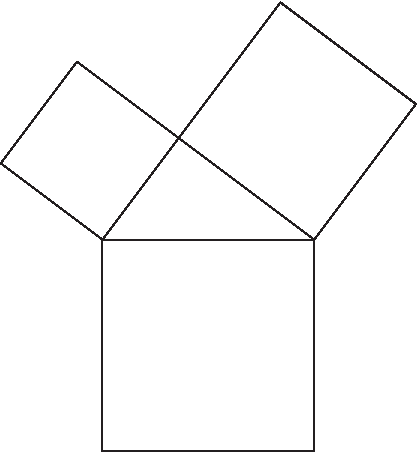
\includegraphics[width=200pt]{pitagora}
\caption[teor. di Pitagora]{Triangolo rettangolo}
\label{figura:pitagora}
\end{center}
\end{figure}

Esistono anche modi per far girare i testo attorno alle
figure. Chi vuole consulti i manuali.

Osservate comunque che in questo stile i paragrafi nelle dimostrazioni non hanno rientro\index{paragrafi, rientro dei} e c'è un quadratino\index{dimostrazioni, quadratino di fine} alla fine.
\end{proof}

\begin{definizione}\label{def:liminfinito}
Si dice che la successione reale $x_n$ tende\index{limite di successioni}\index{successioni, limite di} a~$+\infty$ se per ogni~$M\in\R$ esiste $n_M\in\N$ tale che per ogni~$n\ge n_M$ si ha che $x_n\ge M$.
\end{definizione}

Possiamo riferirci alla definizione~\ref{def:liminfinito}
tramite la sua etichetta\index{etichette}. Il riferimento sarà ``cliccabile'' se si è caricato il pacchetto \verb!uniudtesi! (il quale chiama a sua volta \verb!hyperref!.\index{ipertesto})

\section{Formule}

Anche le formule si possono etichettare:
\begin{equation}
  \label{eq:binomio}
  a+b\,.
\end{equation}
La formula precedente dovrebbe essere la~\ref{eq:binomio} (cliccabile). Non è obbligatorio numerare tutte le formule. Le formule non numerate\index{numerazione formule}\index{formule, numerazione delle}\index{numerazione delle formule} si ottengono o con doppi dollari\index{dollari, doppi}:
$$\dot x\quad
  \ddot x\quad
  \dddot x\quad
  \ddddot x$$
o con l'asterisco\index{asterisco}:
\begin{equation*}
  \overset{\circ}{A}\quad
  \overset{*}{X}\quad
  \vec{x}
\end{equation*}
Testo\index{formula, testo nella}\index{testo nella formula} mescolato a una formula:
\begin{equation}
  x+y=1\text{ quindi }(x+y)^2=1
\end{equation}
$$(x+y)^2\ge0\quad\text{ per ogni }x,y\in\R$$
Carattere grassetto\index{grassetto matematico} matematico:
$$\boldsymbol{y}
  $$
Allineamento\index{allineamento delle formule}\index{formule, allineamento delle} di formule e tre modi di indicare la congruenza\index{congruenze} modulo~$n^2$, con la seconda e terza formula numerate\index{formule, numerazione delle}\index{numerazione delle formule}:
\begin{align}
     u & \equiv  v+1 \pmod{n!}\nonumber \\
     u & \equiv v+1 \mod{n^2} \\
     u & \equiv v+1 \pod{n^2}
  \end{align}
Una formula spezzata\index{formula, spezzamento su righe diverse}\index{spezzamento di una formula su righe diverse} su due righe, ma trattata come un tutt'uno per il numero\index{formule, numerazione delle}\index{numerazione delle formule} di formula:
\begin{equation}
  \begin{split}
    f(x)  :={}& \int_0^{+\infty}t^{x-1}e^{-t}\,dt+\\
         &{}+e^{-x}
  \end{split}
\end{equation}
Due modi di scrivere le frazioni\index{frazioni}:
\begin{equation}
  \frac{1}{2}
  \quad\frac{1}{2}\,.
  \end{equation}
Una definizione per casi\index{casi, definizione
per}\index{definizione per casi}:
\begin{equation}
  f(x):=
  \begin{cases}
    x^2 & \text{se } x\ge0 \\
   -x^2 & \text{se }x<0
  \end{cases}
\end{equation}
Matrici\index{matrici} con e senza parentesi\index{parentesi}:
\begin{equation*}
  \begin{matrix}
    0 & 1 \\
    1 & 0
  \end{matrix}\quad
  \begin{pmatrix}
    0 & 1 \\
    1 & 0
  \end{pmatrix}
  \quad
  \begin{vmatrix}
    0 & 1 \\
    1 & 0
  \end{vmatrix}
\end{equation*}
Due formule di seguito senza allineamento\index{formule, allineamento delle}\index{allineamento delle formule}:
\begin{gather}
  (a+b)^2=a^2+2ab+b^2\label{eq:quadrato} \\
  (a+b)(a-b)(a^2+b^2)=a^4-b^4
\end{gather}

Un esempio di tavola\index{tavola}:

\begin{center}
\begin{tabular}{||l|lr||} \hline
gnats & gram & \$13.65 \\ \cline{2-3}
      & each &      .01 \\ \hline
gnu   & stuffed & 92.50 \\
    \cline{3-3}
emu   &      & 33.33 \\ \hline
armadillo & frozen & 8.99 \\ \hline
\end{tabular}
\end{center}

\appendix

%!TEX TS-program = pdflatex
%!TEX root = tesi.tex
%!TEX encoding = UTF-8 Unicode



\chapter{Come si fanno le appendici}
  
    \index{appendici}
    
    Le appendici si fanno con \verb!\appendix! seguito da
    \verb!\chapter{...}!

%%%%%%%%%%%%%%%%%%%%%%

\chapter{Esempi di Citazioni Bibliografiche}
  
    \index{bibliografia}
    \index{citazioni}
    
    P\^{y}r{\l}å in~\cite{pyrl} ha poi
    generalizzato i risultati di
    Bi\v{s}ker~\cite{bisker1}.
    
    Il pacchetto \verb!uniudtesi! carica
    automaticamente \verb!hyperref!\index{ipertesto},
    che a sua volta rende ``cliccabili'' i riferimenti 
    bibliografici nel documento elettronico.

%%%%%%%%%%%%%%%%%%%%%%

\chapter{Ambiente GNU/Linux (ad esempio Ubuntu)}

    \index{Linux}
    
    \begin{flushright}Contributo di\\ Leonardo Taglialegne
    \end{flushright}
    
    Gli ambienti GNU/Linux contengono parecchi strumenti utili per
    la stesura di una tesi di laurea, in particolare segnaliamo:
    \begin{itemize}
     \item Kile
     \item KBibTeX
    \end{itemize}
    Il primo è un editor per il \LaTeX, che include una tabella
    dei simboli, la visualizzazione della struttura, evidenziazione
    del codice e simili comodità, e nelle ultime versioni fornisce
    una visualizzazione in anteprima dei risultati di compilazione.
    
    Il secondo è uno strumento di ricerca, modifica ed inserimento
    di citazioni in formato BibTeX.
    
    I pacchetti relativi (ed altri utili) si installano,
    su ambienti Debian e Ubuntu con:
    \texttt{sudo apt-get install kile kile-l10n kbibtex
           texlive-science \\
           texlive-math-extra texlive-lang-italian }


\backmatter

%!TEX TS-program = pdflatex
%!TEX root = tesi.tex
%!TEX encoding = UTF-8 Unicode


\begin{thebibliography}{3}
\selectlanguage{english}
\frenchspacing

\bibitem{bisker1}
J. Bi\v{s}ker, \emph{On the elements
of the empty set}. Mathematica Absurdica
\textbf{132} (1999), 13--113.

\bibitem{pyrl}
U. P\^{y}r{\l}\aa, \emph{Generalization
of Bi\v{s}ker's theorem}. Paperopolis
J. Math. \textbf{14} (2001), 125--132.

\end{thebibliography}
\selectlanguage{italian}
\nonfrenchspacing

% \printindex % se si fa l'indice analitico.

\end{document}
